\chapter{Virtual Private Cloud (VPC)}\label{ch:vpc}

Amazon VPC allows for AWS resources to be launched in a virtual network that has been custom defined and configured.
This virtual network is similar to a traditional network which operates within your own physical data center, with the
added benefits of the scalable AWS infrastructure~\parencite{amazon2022what}.
A VPC can have multiple assigned subnets, which are a range of IP addresses accessible in the VPC\@.

The first step of migrating the web app to the cloud was creating a VPC to deploy and manage AWS resources for the app.
To do this, the VPC wizard must be used.
This is accessed by navigating to the VPC Management Console and then click the Launch VPC Wizard button, which can be
seen in Figure~\ref{fig:vpc-wizard}.

\begin{figure}[!htbp]
    \centering
    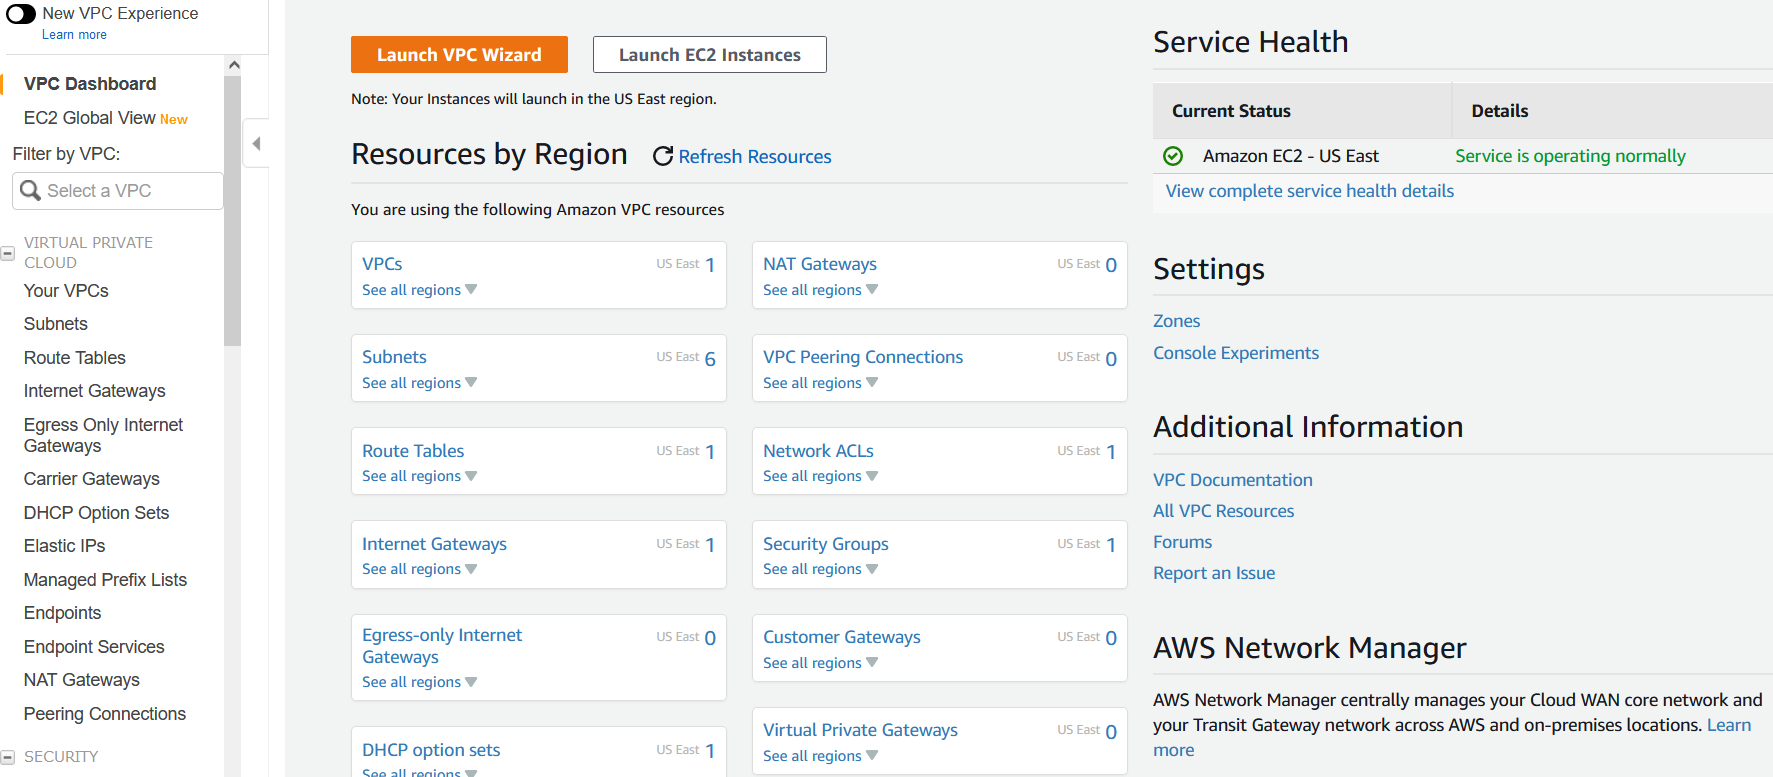
\includegraphics[width=\textwidth]{resources/vpc/vpc-dashboard}
    \caption{VPC Management Console.}
    \label{fig:vpc-wizard}
\end{figure}

The wizard presents us with step one of creating a VPC: selecting a VPC configuration.
There are several options for this, where each configuration has the following features:

\begin{itemize}
    \item VPC with a Single Public Subnet: Creates a /16 network with a /24 subnet where the subnet instances use
    Elastic IPs or Public IPs for internet access.
    \item VPC with Public and Private Subnets: Creates a /16 network and two /24 subnets where the public subnet
    instances use Elastic IPs for internet access and the private subnet instances use NAT for internet access.
    \item VPC with Public and Private Subnets and Hardware VPN Access: Creates a /16 network with two /24 subnets where
    one subnet is connected to the internet and another is connected to your personal network via a VPN\@.
    \item VPC with a Private Subnet Only and Hardware VPN Access: Creates a/16 network and a /24 subnet where the
    subnet is connected to your personal network via a VPN\@.
\end{itemize}

For the deployment of this web app, hardware VPN access is not necessary, so the VPC configuration with public and
private subnets was selected, as seen in Figure~\ref{fig:vpc-step-1}.

\begin{figure}[!htbp]
    \centering
    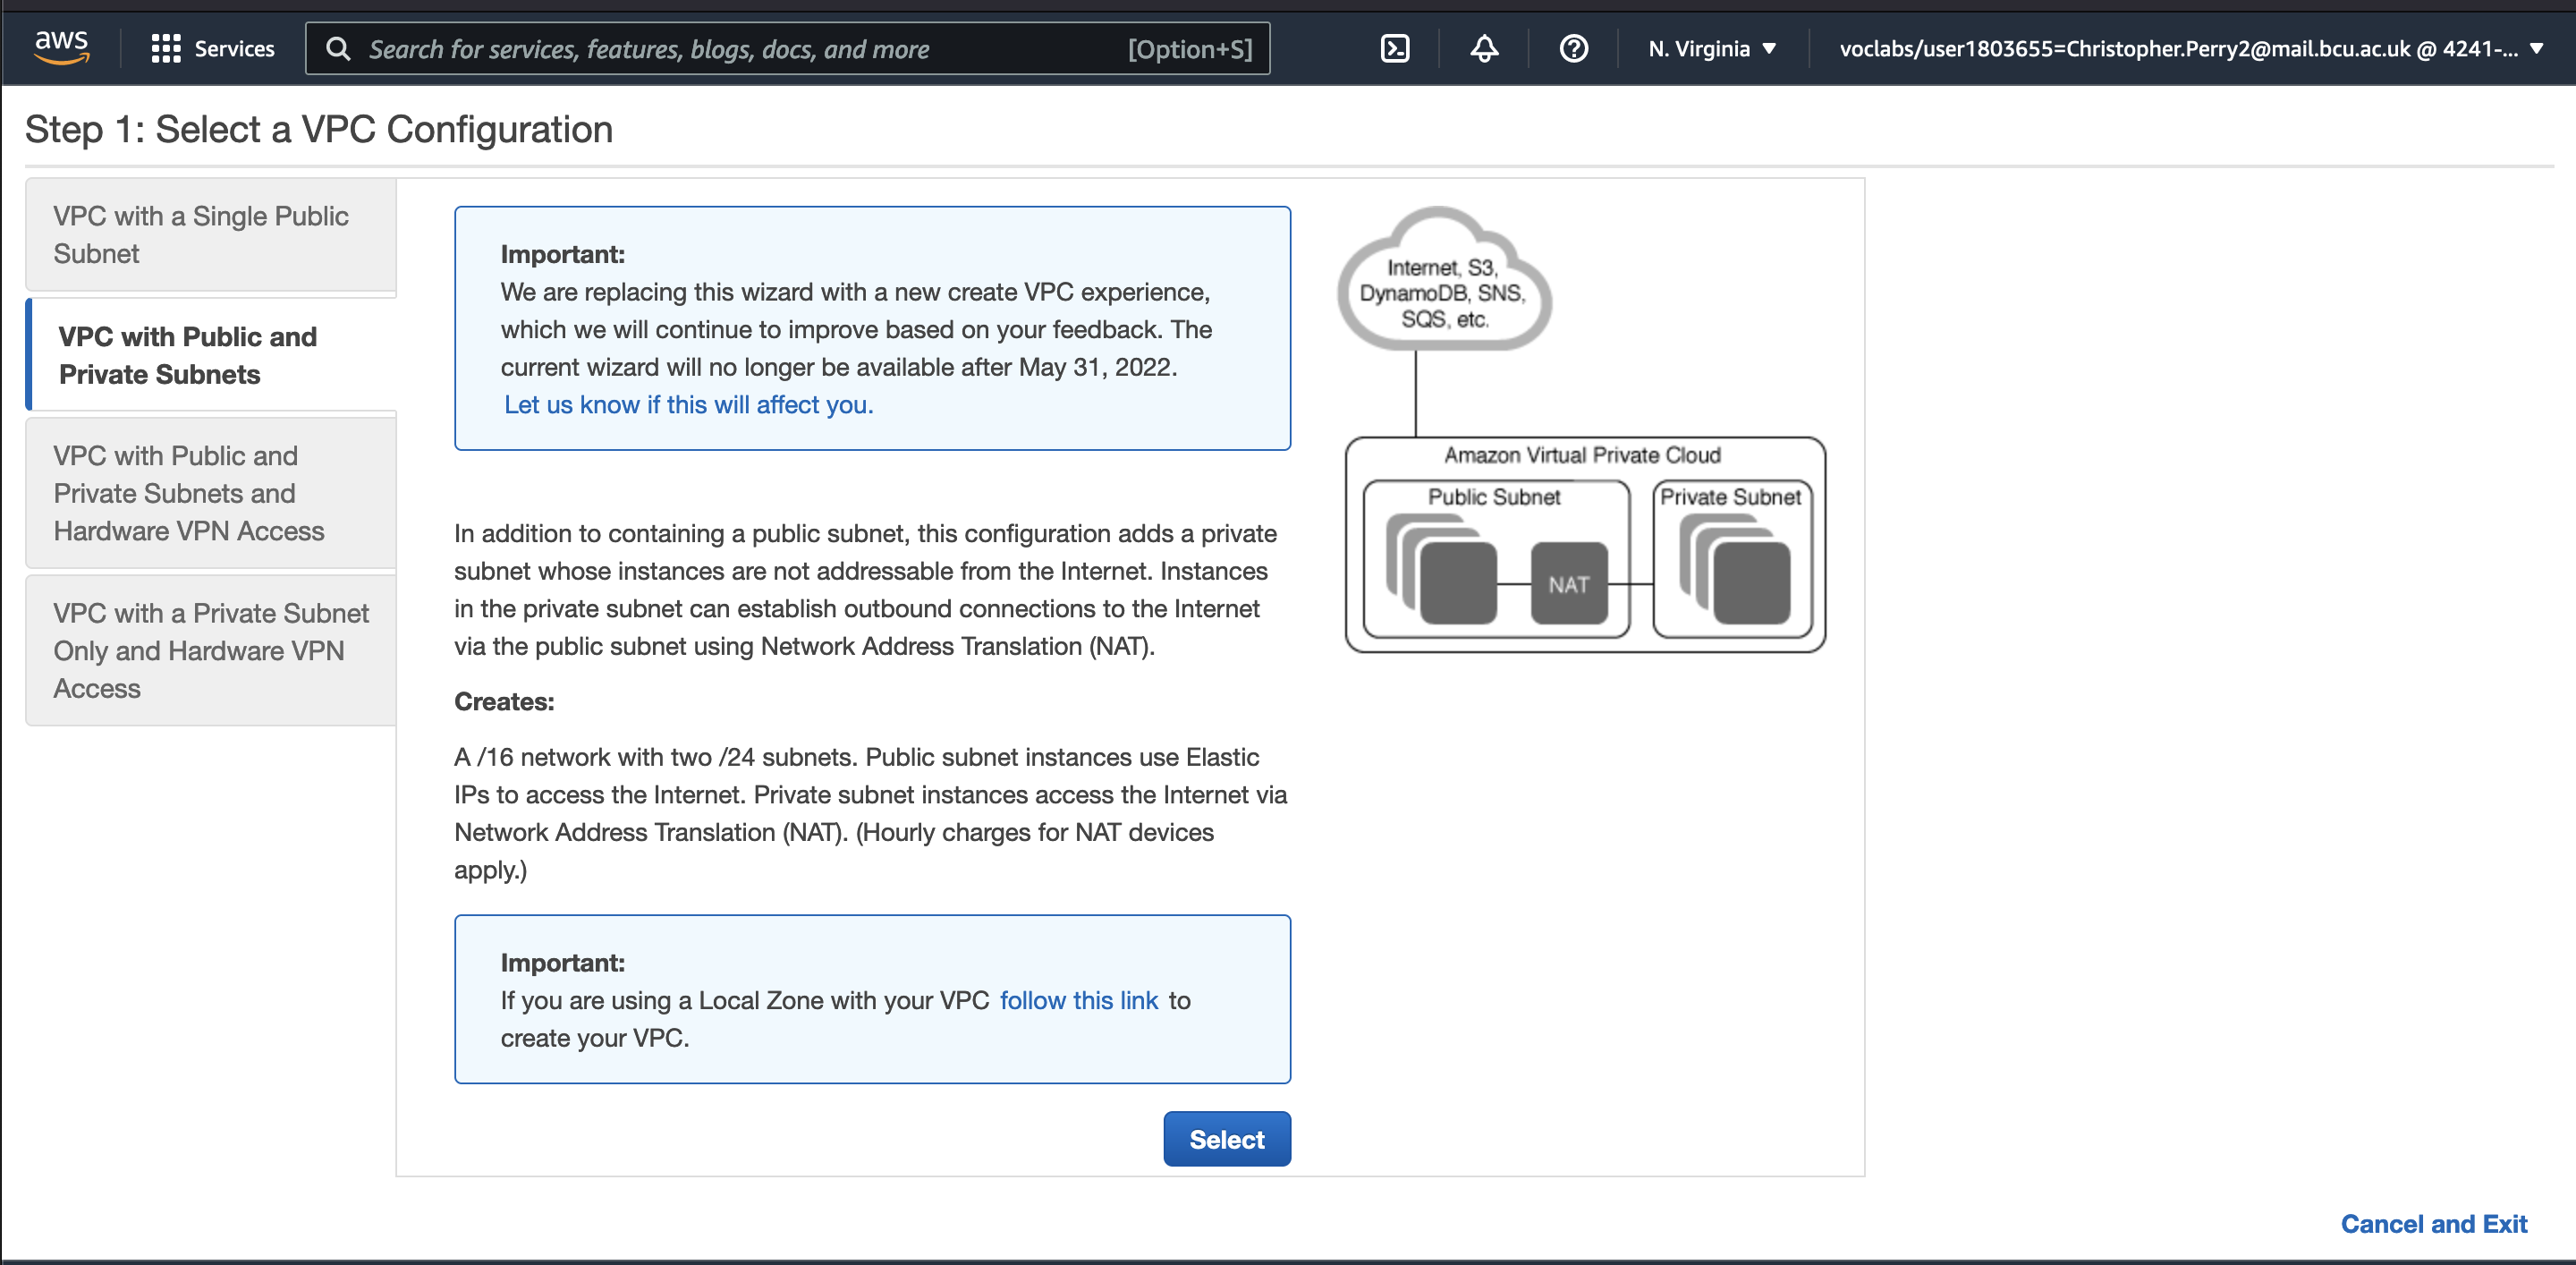
\includegraphics[width=\textwidth]{resources/vpc/step_1_select_a_vpc_configuration}
    \caption{Selecting a VPC configuration.}
    \label{fig:vpc-step-1}
\end{figure}

Following this, the specific details, such as the IP address block, of the selected configuration must be entered.
An IPv4 CIDR block of \mintinline{zsh}|10.0.0.0/16| was chosen as it provides a large amount of available IP addresses.
Additionally, no IPv6 CIDR block was configured and the VPC was named \mintinline{zsh}|Group4_VPC|.

Next, the public and private subnets were configured.
The public subnet was assigned an IPv4 CIDR of \mintinline{zsh}|10.0.0.0/24|, making 251 distinct IP addresses available
for the public subnet.
The availability zone of \mintinline{zsh}|us-east-1a| was chosen and the subnet was named
\mintinline{zsh}|Public subnet 1|.
The private subnet was assigned an IPv4 CIDR of \mintinline{zsh}|10.0.1.0/24|, making 251 distinct IP addresses
available for the private subnet as well.
The availability zone of \mintinline{zsh}|us-east-1a| was chosen and the subnet was named
\mintinline{zsh}|Private subnet 1|.

Lastly, the previously created Elastic IP Allocation ID was selected, and the remaining settings were left at their
default values.
Clicking the Create VPC button now will generate the VPC with the specified configurations.

\begin{figure}[!htbp]
    \centering
    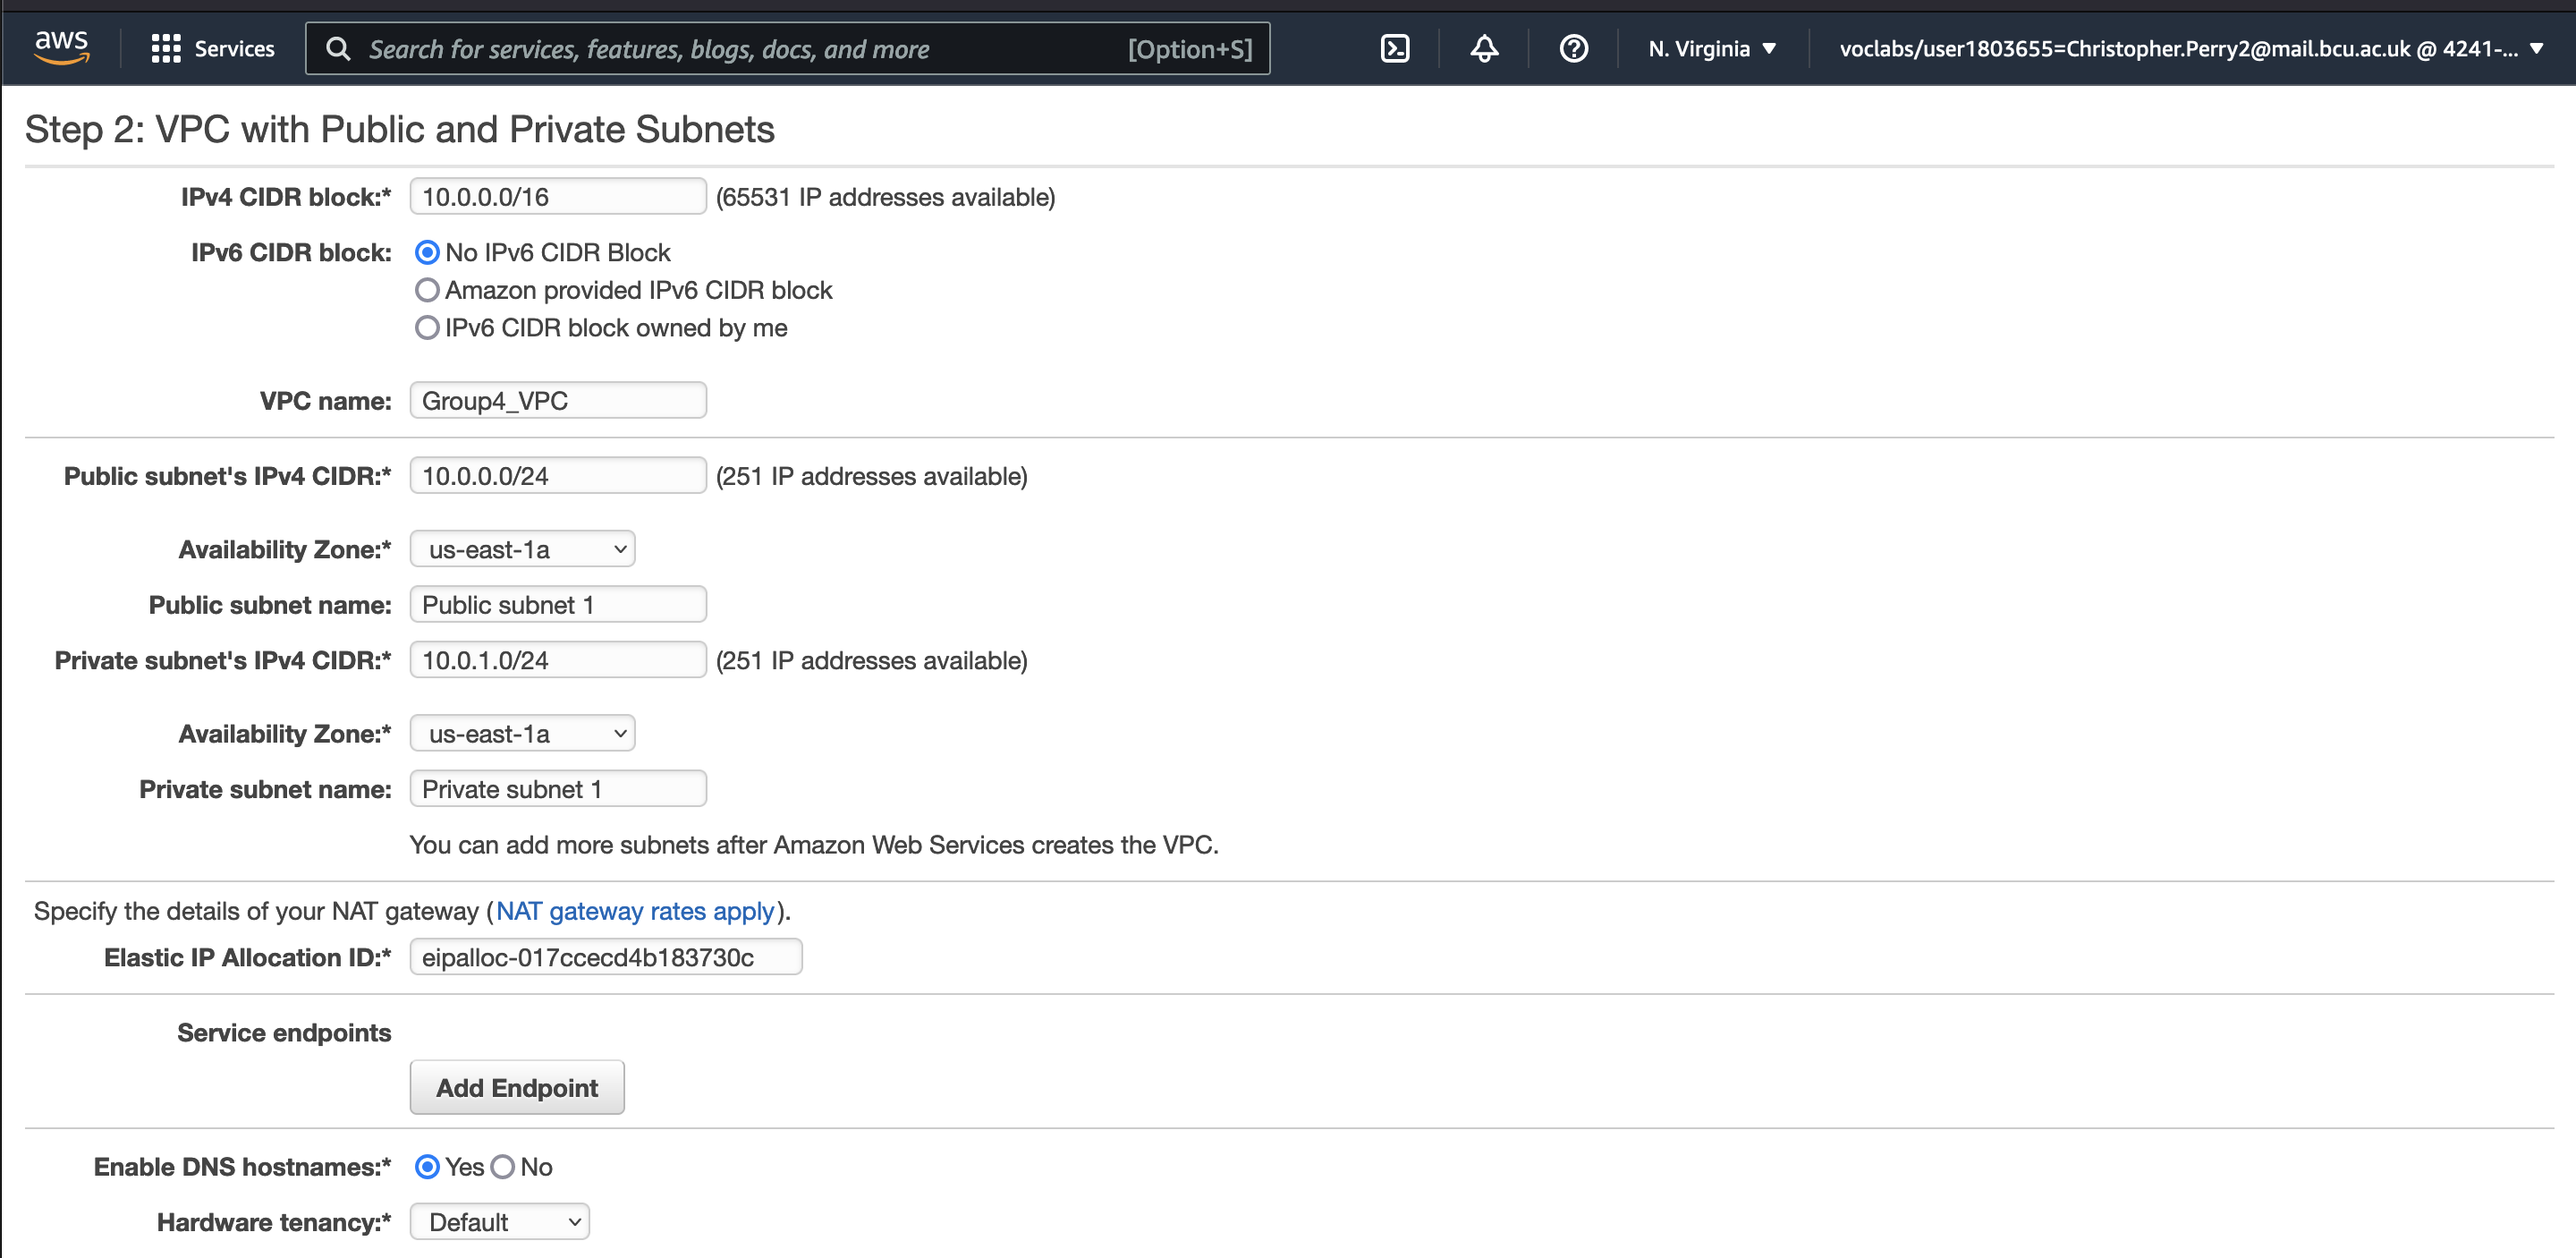
\includegraphics[width=\textwidth]{resources/vpc/step_2_vpc_with_public_and_private_subnets}
    \caption{Configuring VPC public and private subnets.}
    \label{fig:vpc-step-2}
\end{figure}

After this, AWS takes a few minutes to generate the VPC\@.

\begin{figure}[!htbp]
    \centering
    
\includegraphics[width=\textwidth]{resources/vpc/step_3_create_vpc}
    \caption{Generating the VPC.}
    \label{fig:vpc-step-3}
\end{figure}

\begin{figure}[!htbp]
    \centering
    
\includegraphics[width=\textwidth]{resources/vpc/step_3_create_vpc}
    \caption{Generating the VPC.}
    \label{fig:vpc-step-3}
\end{figure}